\section{Introdução}
\subsection{Teoria da Informação}
\begin{frame}%[allowframebreaks]
  \frametitle{Teoria da Informação e Codificação}

    \begin{itemize}[<+->]
    \item Surgiu em 1948 com a publicação do trabalho ``The Mathematical Theory of Communications'' \cite{shannon1948}.
    \item Teoria da Informação lida com as limitações teóricas e potencialidades de sistemas de comunicação.
    \item O que é informação? Como mensurar?
    \item Codificação. Como representar uma informação?
    \item Canal de Comunicação.
    \end{itemize}

\end{frame}
\note{
    \small
    \begin{itemize}
	\item A distinguibilidade entre as mensagens é fator importante para caracterizar informação.
        Pela definição de Shannon, ``Informação é a habilidade de distinguir de forma confiável
        dentre um rol de alternativas possíveis''.
	\item O problema central em Teoria da Informação é a transmissão eficiente e confiável de dados, 
	do transmissor a um receptor, através de um canal de comunicação.
	\item Eficiência (usar o mínimo de recursos possível).
	\item Confiabilidade (evitar erros, ser capaz de detectá-los e corrigi-los).
	\item A informação é um conceito paradoxal. Por um lado necessita de uma representação física,
        por outro lado é abstrata. Uma mesma informação pode ser representada em papel,
        em um meio magnético ou ótico, pode ser representada por ondas mecânicas ou elétricas.
        \item Linguagem. Comunicação falada e escrita. Código faz associação entre símbolo e mensagem
	e é `arbitrário'.
    \end{itemize}
}
\note{
    \small
    A área da ciência criada por Shannon ampliou-se ao longo do tempo e influência diversas outras áreas.
    Por exemplo: teoria da comunicação, criptografia, ciência da computação, física (mecânica estatística),
    matemática (probabilidade e estatística), filosofia da ciência, linguística e processamento de linguagem natural,
    reconhecimento de fala, reconhecimento de padrões e aprendizado de máquina, compressão de dados, economia,
    biologia e genética, psicologia, etc.

    \vspace{3ex}
    Shannon entrou para o Bell Labs para trabalhar com sistemas de controle de disparo
    e criptografia durante a Segunda Guerra Mundial, sob um contrato com o Comitê Nacional de Pesquisa para Defesa
    Em 1945, Shannon elaborou um memorando sigiloso, que posteriormente foi publicado sob o título
    ``Communication Theory of Secrecy Systems''. Este incorporava muitos dos conceitos e formulações matemáticas
    do artigo mais consagrado ``A Mathematical Theory of Communication'' (1948).
}
\note{
    \small
    \begin{itemize}	
	\item Codificação - criar códigos com algoritmos práticos para codificação e decodificação para
	serem utilizados na comunicação no mundo real em canais ruidosos.
	\item Exemplos de codificações conhecidas para representar informação: código Morse, código ASCII, etc.
    \end{itemize}
}

\begin{frame}%[allowframebreaks]
  \frametitle{Código Morse}
  \hvFloat[floatPos=htb,capPos=right,capVPos=bottom,objectPos=c]{figure}{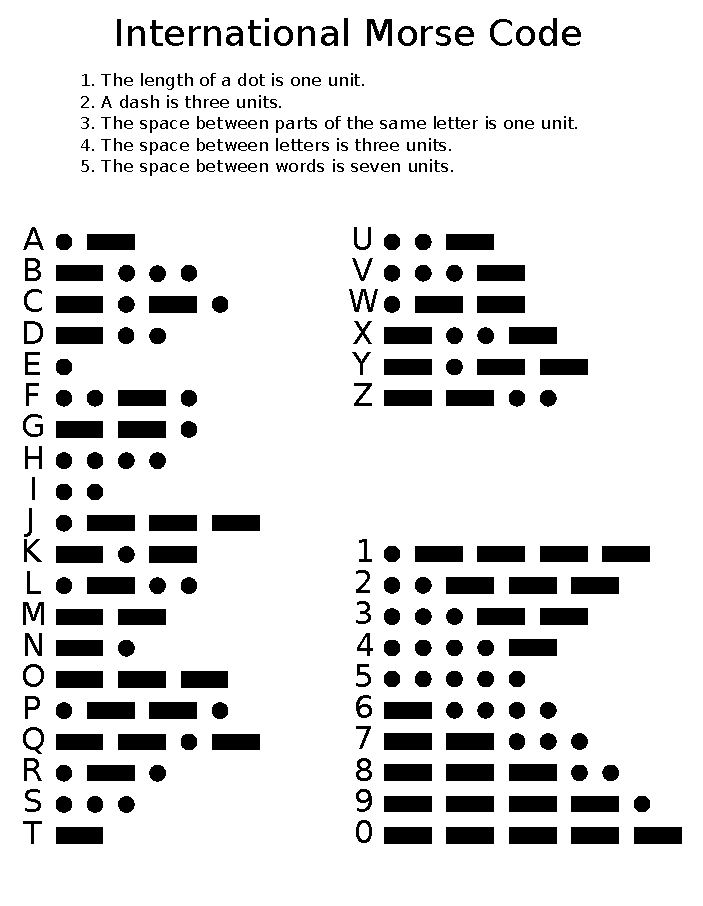
\includegraphics[trim=0cm 0cm 0cm 3.5cm,clip=true,width=0.45\textwidth]{images/International_Morse_Code.pdf}}
  {Código Morse internacional (\cite{wiki:morse}). Letras do alfabeto ordenadas por frequência de ocorrência no inglês: etaoin shrdlu cmfwyp vbgkjq xz (\cite{wiki:etaoin,wiki:letterfreq}).}{fig:morse}
\end{frame}

\begin{frame}%[allowframebreaks]
  \frametitle{Código Unário}
  Claude Mendibil utilizou o código unário (1, 01, 001, 0001, ...) 
  para representar as letras do alfabeto ESARINTULOMDPCFBVHGJQZYXKW.
  Utilizando este código, Jean-Dominique Bauby ditou o livro \textit{Le Scaphandre et le Papillon} (O Escafandro e a Borboleta).
  \hvFloat[floatPos=htb,capPos=right,capVPos=bottom,objectPos=c]{figure}{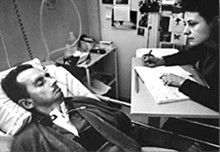
\includegraphics[width=0.45\textwidth]{images/bauby.jpg}}
  {Foto de Bauby em 1996 ditando suas memórias para Claude Mendibil (\cite{wiki:bauby}).}{fig:bauby}
\end{frame}


